
Statistical techniques play a central role in high-energy physics, as they provide the tools needed to interpret, quantify, and extract meaningful information from the experimental results obtained at the LHC. This chapter outlines the different statistical methods employed throughout this thesis. A frequentist approach is adopted, in which the concept of probability refers to the relative frequency of an outcome in a repeatable experiment.

First, the statistical modelling of experimental data is introduced, including the construction of the likelihood function for binned data and the treatment of systematic uncertainties through nuisance parameters. This modelling stage provides the essential ingredients subsequently used for the statistical inference, which allow us to extract physics results from the data, including parameter estimation and hypothesis testing. The framework used for building and implementing these statistical models is \textsc{TRExFitter}~\cite{trexfitter}, which relies on the \textsc{HistFactory}~\cite{histfactory} format and the \textsc{RooFit}~\cite{roofit} and \textsc{RooStats}~\cite{roostats} environments for model definition and statistical interpretation.

Finally, the use of multivariate techniques is discussed to perform classification and improve signal-to-background separation. In particular, an introduction to supervised learning and the machine learning algorithms used in this work is provided, with a focus on deep neural networks (DNNs) and boosted decision trees (BDTs). The increasing relevance and application of such techniques in particle physics reflects their ability to model complex correlations between observables, offering substantial improvements in classification and analysis optimisation tasks.

\section{Statistical Modelling}
\label{sec:stat_modelling}
% Aquí irán aspectos relacionados con la construcción de modelos estadísticos,
% likelihoods, parámetros, modelado de fondo/señal, etc.

\section{Statistical Inference}
\label{sec:stat_inference}
% Aquí se incluirán conceptos sobre estimadores, verosimilitud, p-valores, intervalos de confianza,
% tests de hipótesis, profile likelihood, significancia, etc.

\section{Machine Learning Techniques}
\label{sec:ml_methods}
This section provides a general overview of the two most relevant algorithms used and developed throughout this thesis: DNNs and BDTs. Usually encompassed under the term multivariate techniques, these are machine learning algorithms that offer excellent performance in the tasks to which they have been applied.
Most of concepts here presented are taken from reference~\cite{Goodfellow-et-al-2016}

In general terms, a machine learning algorithm can be defined as one that is capable of learning to perform a specific task based on input data, which typically consists of a multidimensional set of features. This thesis focuses specifically on supervised machine learning algorithms, which are trained using a set of $n$ input data elements, $X = \left\{\vec{x_{0}}, \vec{x_{1}}, ..., \vec{x_{n}} \right\}$, where each element encapsulates $m$ features, as previously mentioned, $\vec{x_{i}}=(x_{i,0}, x_{i,1}, ..., x_{i,m})$. The term "supervised" is used because each data point is associated with a known true label $y_{i}$, and the goal is to infer this label for new, unseen data using the input provided during training.

\subsubsection*{Datasets preparation}
When training a supervised machine learning model, the so-called training dataset is used to optimize the model parameters. However, in order to properly evaluate the model's performance and select its best version, one must rely on data that has not been seen during the training process. If the same training dataset were used for evaluation, the model could learn overly specific features or fluctuations from this subset that are not present in real experimental data. This would ultimately lead to degraded performance when applied to unseen data. This issue is known as overtraining or overfitting.

To mitigate this problem and improve generalization, a validation dataset is used. The model's performance is monitored on this separate dataset during training in order to guide the optimization process and prevent overfitting. The version of the model that performs best on the validation data is typically chosen as the final one.

For a final, unbiased evaluation of the model’s performance, a third dataset, called test dataset, is employed. Since both the training and validation datasets have already influenced the model, they cannot be used to assess its final quality. Typically, the three datasets (training, validation, and test) are obtained from the same original input sample by randomly splitting its data points.

Another widely used approach to maximize the use of available data is the \textit{k-fold} cross-validation technique~\cite{tmvatoolkit}. In this method, the original dataset is split into $k$ equal parts (or "folds"). The model is then trained $k$ times, each time using $k\minus1$ folds for training and the remaining one for validation. This allows every data point to be used for both training and validation at different stages, providing a more robust performance estimate and making efficient use of limited datasets.

\subsubsection*{Type of prediction}
A ML algorithm can be designed to perform various tasks, even multiple ones simultaneously. These include data synthesis and sampling, anomaly detection, and others. Many of these tasks are also employed in the context of high energy particle physics.
In this thesis, we focus specifically on classification, the most fundamental task besides regression.

Classification problems generally involve that the learning algorithm is asked to determine which of $k$ predefined categories a given input belongs to. Formally, this is often expressed as finding a function $f: \mathbb{R}^n \rightarrow \{1, \dots, k\}$, where a vector of input features $\vec{x}$ is assigned a class label $y = f(\vec{x})$. In many practical implementations, especially in physics applications, the model does not directly return a class label, but instead provides a probability distribution over all possible classes. The final classification decision can then be made by selecting the class with the highest predicted probability.

If $k = 2$, the task is referred to as binary classification, and the model typically outputs a single value representing the probability that the input belongs to one of the two classes (e.g., signal vs background in our domain). The probability of the alternative class is simply $1 - f(\vec{x})$. If $k > 2$, the task is referred to as multinomial classification and in such cases, one probability is returned for each class and the outputs can be combined into a single discriminant using a likelihood ratio as prescribed by the Neyman-Pearson lemma~\cite{Neyman:1933wgr}:
\begin{equation}
    \frac{p_0}{\sum_{i=1}^k f_i p_i},
\end{equation}
where $p_i$ is the predicted probability for class $i$ and $f_i$ is a configurable weight that adjusts the importance of each class in the denominator. By tuning the $f_i$, the classifier’s sensitivity to specific backgrounds or categories can be adjusted to fit the needs of a particular analysis.

\subsubsection*{Loss function}
To quantify the optimization of a supervised machine learning model during its training, it is necessary to measure how well it is performing. For this purpose, a loss (or cost) function is defined, which is the function to be minimized during the training of the model.  
The loss function of a dataset is computed by evaluating the loss value on each data point and averaging over all points:
\begin{equation}
    \mathcal{L}(\hat{\vec(y)},\vec(y)) = \frac{1}{N}\sum^{N}_{i=1} \mathcal{L}(\hat{y}_{i},y_{i}),
\end{equation}
where the $\hat{\vec{y}}$ are the set of predictions made by our model, and ${\vec{y}}$ are the corresponding true labels, $N$ is the number of data points in our dataset. $\mathcal{L}$ is our loss function, and the choice we make for it will depend on the problem we are dealing with, leading to more or less efficient solutions.
When we talk about a regression problem, the simplest one, like a linear fit of a straight line, the Mean Absolute Error (MAE) is commonly used, $\mathcal{L}(\hat{y},y) = |\hat{y} - y|$.
For binary classification, the most commonly used loss function is the so-called binary cross-entropy, $\mathcal{L}(\hat{y},y) = -y\log(\hat{y}) + (1-y)\log(1-\hat{y})$.
Its generalization to the case of multinomial classification is obtained through the categorical cross-entropy, defined as:
\begin{equation}
    \mathcal{L}(\hat{y},y) = - \sum_{c} y_{c} log(\hat{y}_{c}),
\end{equation}
being $c$ each of the classes considered in the problem.

\subsubsection*{Performance measurements}

As mentioned earlier, the final performance of the trained model must be tested on a totally unseen test dataset. The loss function primarily serves to guide the optimization process during training, although a low final value often indicates the goodness of our model. Specific metrics or figures of merit, depending on the problem at hand, are usually employed to gain a deeper understanding of the efficiency of our ML models.

In the case of classification problems, as in our work, the most commonly used figure of merit is the Receiver Operating Characteristic (ROC) curve, which provides a clear visualisation of the performance of a binary classifier in terms of signal and background identification efficiency, which is precisely the core issue we aim to address.

We aim to optimise both quantities, and to obtain the ROC curve we compute them for different values of the discriminant output of our algorithm. The signal identification efficiency is calculated as the number of candidates with a discriminant value above the threshold, divided by the total number of signal candidates. Instead of background efficiency, we typically use its inverse: the background rejection. Plotting background rejection against signal efficiency allows us to identify the model that offers the best performance, as illustrated in the example in Figure~\ref{fig:roc_curves}. The optimal model will be the one that reaches values closest to the upper right corner.

\begin{figure}[htbp]
    \centering
    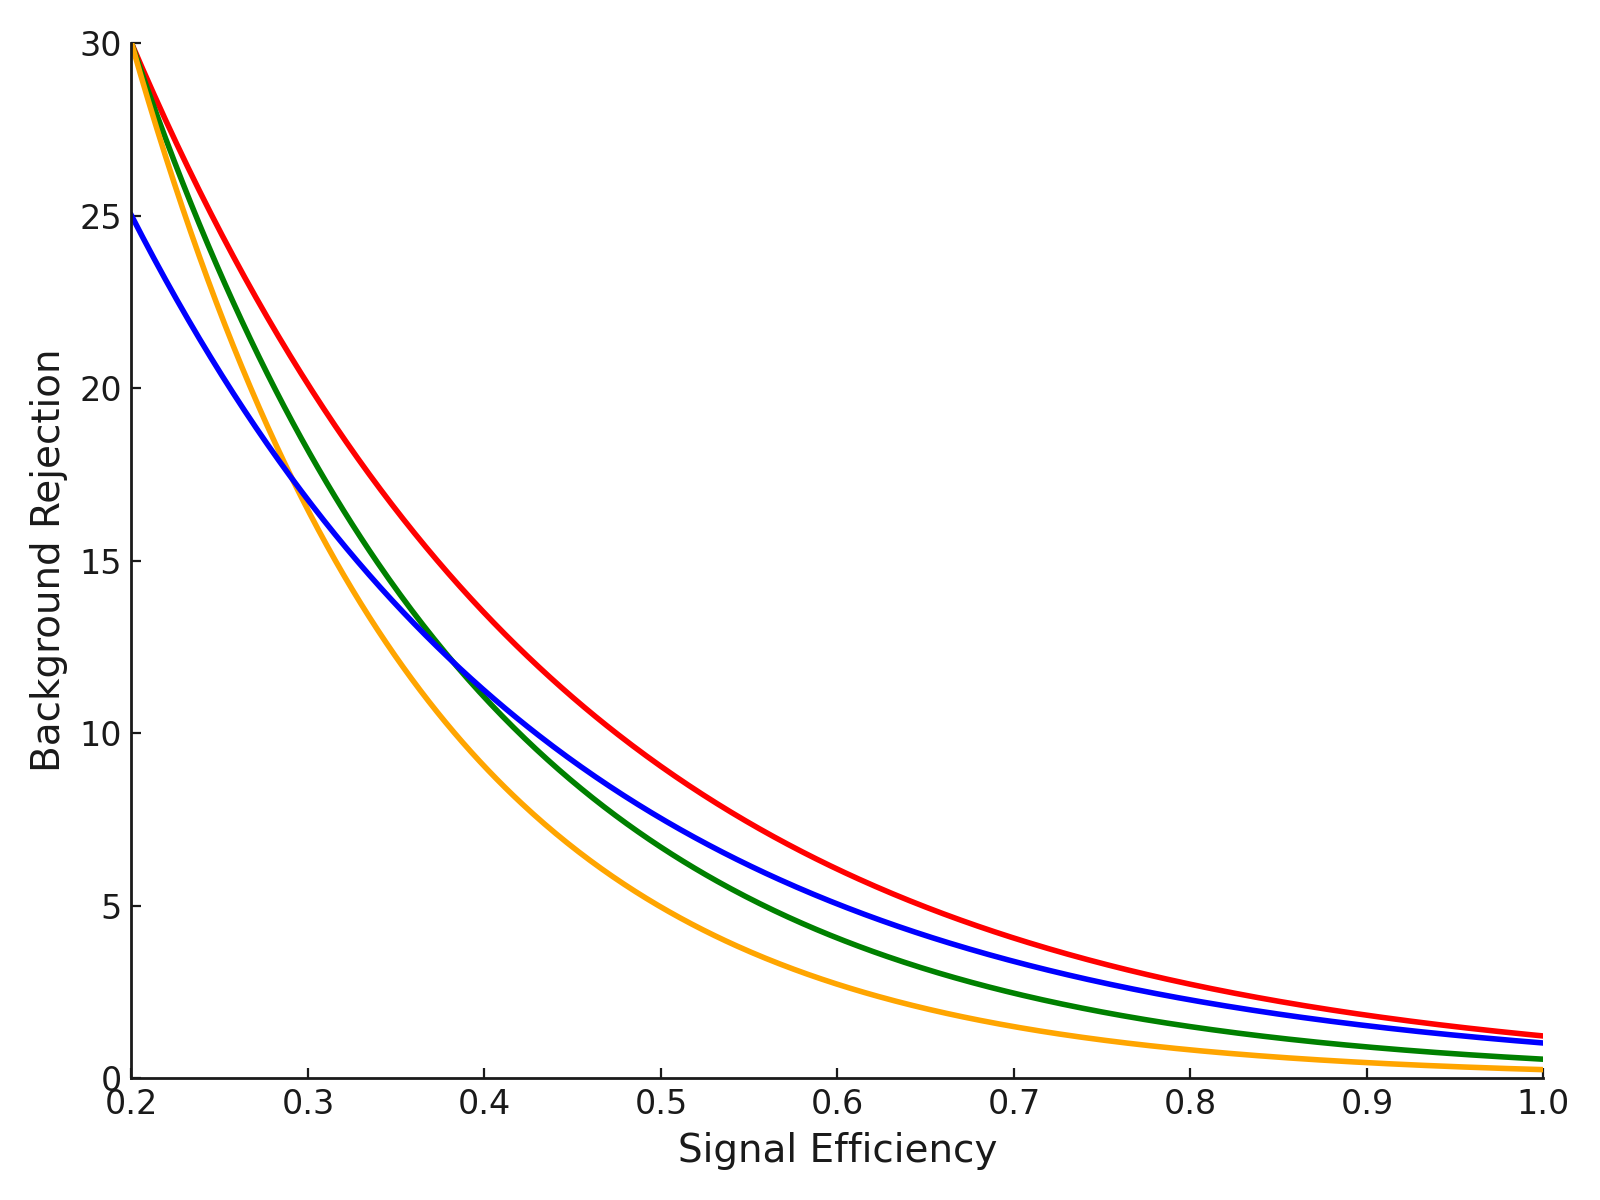
\includegraphics[width=0.7\textwidth]{images/roc_curves_clean.png}
    \caption{Example of ROC curves evaluated for different models in terms of signal efficiency and background rejection.}
    \label{fig:roc_curves}
  \end{figure}

\subsection{Deep Neural Networks}
\label{subsec:dnn_general}
% Esta sección contendrá los fundamentos de las DNN: arquitectura, función de activación,
% función de pérdida, entrenamiento, regularización, overfitting, etc.
% Será genérica y no específica de electron ID, para poder referenciarla desde otras secciones.

One of the most widely used and well-known ML algorithms are Neural Networks (NNs). There exists a broad variety of architectures, but the most basic ones are the Deep Neural Networks (DNNs), generally referring to any NN with multiple hidden layers. In this thesis, we implicitly refer to Feed-Forward DNNs, where information flows in one direction, from input to output, without any feedback or recurrence.

In general terms, the simplest form of a NN is a linear layer, which applies an affine transformation to the input data and can be described as:
\begin{equation}
    \vec{x}_{out} = W\vec{x}_{in} + b,
\end{equation}
where $W$ is a weight matrix associated with each node, $b$ is a bias vector, and $\vec{x}_{\text{in,out}}$ are the input and output feature vectors. Both the weights and the biases are parameters learned and optimized by the NN during training.

In the end, to build a DNN, depending on the complexity of the problem, the architecture is constructed by stacking multiple layers, which are applied sequentially, as illustrated in Figure~\ref{fig:dnn}.
\begin{figure}[htbp]
    \centering
    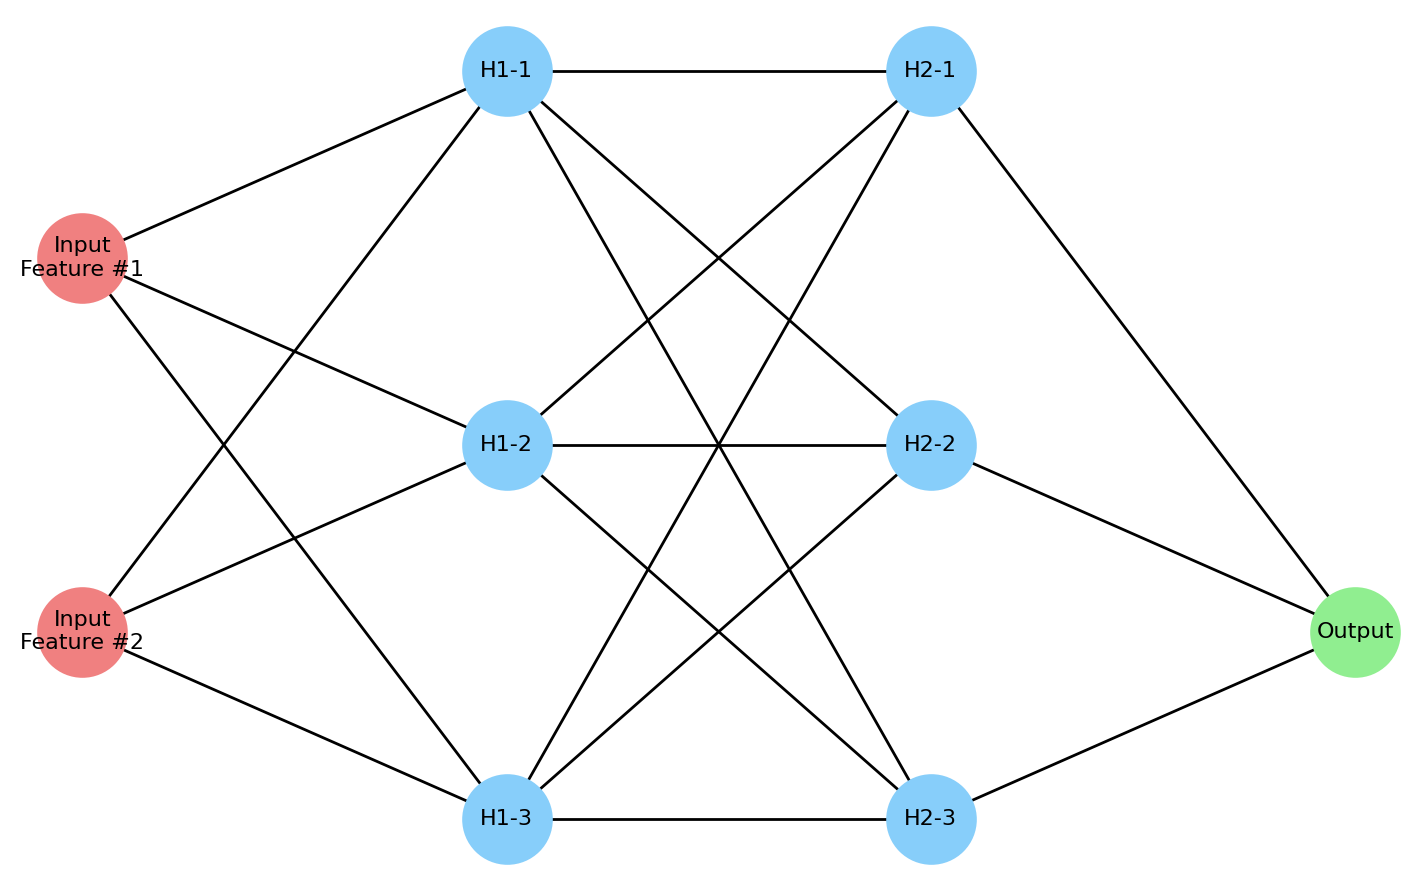
\includegraphics[width=0.7\textwidth]{images/dnn.png}
    \caption{Diagram of Neural Network architecture with two input features, two hidden layers with three nodes each and one output.}
    \label{fig:dnn}
  \end{figure}

It is important to note that the real dependencies and correlations among the input features are very likely to be non-linear and follow more complex patterns. However, since a single layer applies an affine transformation, the output will ultimately remain affine.
To enable the algorithm to learn and handle non-linearities, activation functions are used.

\subsubsection{Activation functions}
Non-linearity is achieved by passing the output of a linear layer through an activation function. One of the most commonly used activation functions is the Rectified Linear Unit (ReLU), which is simply defined as follows
\begin{equation}
    f(x)= \left\{\begin{array}{lcc} x, & if & x \ge 0 \\ 0 & if & x < 0 \\ \end{array}\right}.
\end{equation}

This simple action of setting the unit for positive inputs and zeroing the function otherwise introduces a non-linearity, and its derivative is straightforward to compute, which is beneficial for optimization.  

There are other options that, in certain cases, can improve the performance of the NN output, such as the Leaky Rectified Linear Unit (Leaky ReLU), which modifies the negative part to have a small slope~\cite{Maas2013RectifierNI}, meaning that negative values are not discarded but scaled by a certain factor. Another example is the Gaussian Error Linear Unit (GELU)~\cite{hendrycks2023gaussianerrorlinearunits}. As an illustration, a representation of these activation functions and their derivatives is shown in Figure~\ref{fig:activation}.
\begin{figure}[htbp]
    \centering
    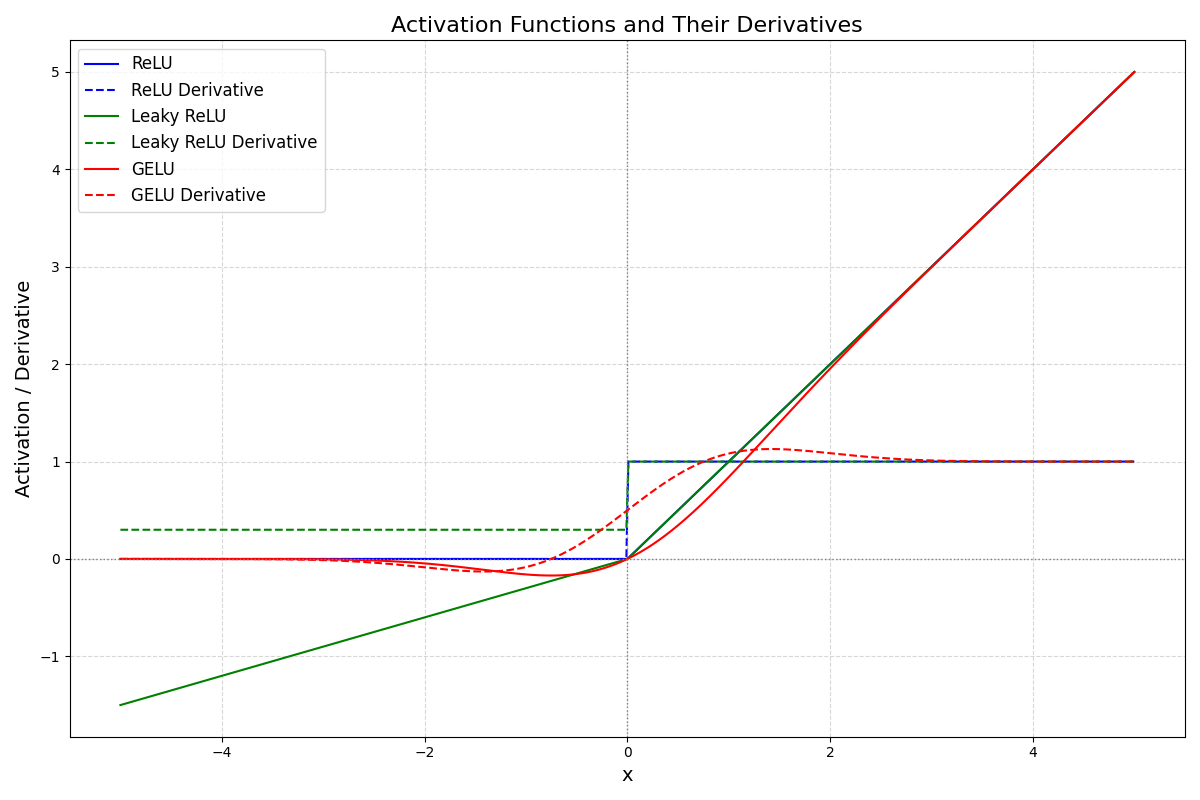
\includegraphics[width=0.7\textwidth]{images/activation_functions.png}
    \caption{Some activation functions and their derivatives: ReLU (blue), leaky ReLU (green, slope of 0.3), GELU (red).}
    \label{fig:activation}
\end{figure}

Another commonly used function is the sigmoid function, which is bounded between 0 and 1, given by
\begin{equation}
  f (x) = \frac{1}{(1 +exp(−x))},
\end{equation}
which is mainly used in the output layer of neural networks built for binary classification, so that the output can be directly interpreted as a probability. The generalisation of this function, called the softmax function, is used when the classification is multinomial and multiple outputs are present. It is defined as:
\begin{equation}
    f (x_{i}) = \frac{exp(x_{i})}{\sum_{j}exp(x_{j})},
\end{equation}
ensuring that the sum of the outputs corresponding to all classes equals 1, and that individual outputs can also be interpreted as the probability of belonging to each class.

\subsubsection{Regularization}

Although regularisation techniques such as L2 regularisation, dropout, or normalisation layers are often employed to mitigate overfitting in neural networks, they are not explicitly used in the training strategy followed in this thesis. Nevertheless, the underlying principle remains the same: to increase the generalisation power of the model and avoid learning noise or fluctuations specific to the training dataset.

In this thesis, batch normalisation~\cite{ioffe2015batchnormalizationacceleratingdeep} is applied as the only regularisation-related technique. Batch normalisation acts by normalising the inputs of each layer to have zero mean and unit variance within a given batch of training data. This standardisation is done feature-wise, helping to stabilise and accelerate the training process. Moreover, it allows the use of higher learning rates and reduces sensitivity to initialisation. Unlike layer normalisation, which computes statistics over all features in a layer for each point separately, batch normalisation computes statistics across the entire batch, making it particularly effective in deep networks trained with mini-batches.

\subsubsection{Optimization and Training}

As previously discussed, the loss function guides the learning process of our neural networks. The optimisable parameters of our algorithm are updated using an optimiser. A wide range of optimisers exists, many of which are based on Stochastic Gradient Descent (SGD), which essentially computes the gradient of the loss function with respect to these parameters.

Aiming to minimise the loss function, the parameters are updated at each step in the negative gradient direction as follows (for a single parameter):
\begin{equation}
    \theta_{i+1} = \theta_{i} - \eta \Delta_{\theta}\mathcal{L}_{\theta}(\hat{\vec{y}},\vec{y}),
\end{equation}
where $\theta_{i}$ is the learnable parameter at step $i$, and $\eta$ is the learning rate (LR), which defines the step size. In this thesis, an extension of the SGD optimiser called $Adam$~\cite{kingma2017adammethodstochasticoptimization} is used.

Since analytical computation of the gradients is infeasible, the backpropagation algorithm~\cite{Rumelhart1986LearningRB} is employed. It efficiently computes these gradients by propagating the computation backwards from the output layer to the input.

Finally, it is during the training itself that the learnable parameters are optimised based on the input data. Information is passed to the algorithm in small subsets of data, called $batches$. The value of the loss function is computed on each batch and used to update the network's parameters, aiming to reduce the loss function as described.

This process is repeated for all the batches into which the original dataset has been divided, completing what is known as one $epoch$. After each epoch, the performance of the neural network is evaluated on the validation dataset. We repeat this for all the agreed number of epochs and finally retain the model that performs best in terms of validation loss.

Regarding the implementation of the architecture and its optimisation, there are many software libraries available for machine learning, with TensorFlow~\cite{tensorflow2015} and PyTorch~\cite{pytorch} being among the most widely used. The neural network model used in this thesis was implemented using TensorFlow version 2 (various minor releases). Since these frameworks are not natively compatible with the ATLAS software environment, the \texttt{lwtnn}~\cite{lwtnn,lwtnn2} package was originally developed to facilitate the integration of neural networks into the ATLAS software.

\subsubsection{Preprocessing}

\subsubsection{Input Data and Preprocessing}
\label{dnn:preprocessing}

A common issue when directly feeding a DNN with the collected training input dataset is that the algorithm might learn specific features that are either irrelevant or not fully representative of what is expected in real data. This can lead to a degradation in performance. To mitigate such effects, a data preprocessing step is introduced before passing the input to the algorithm.

Applying scaling or certain transformations to the input data is generally beneficial in most cases. In general, DNNs tend to perform better when input features are of order one. This significantly improves the stability of the training process, its speed and efficiency, and ultimately the final performance of the algorithm.

A simple way to illustrate this is to consider a neural network with two inputs, $x_{1}=1$ and $x_{2}=100$. In the first hidden layer, each node combines these inputs as $w_{1}x_{1} + w_{2}x_{2}$, where $w_{1}$ and $w_{2}$ are the weights. These typically start with similar values during optimisation, so due to the large difference in the input values, $x_{1}$ contributes very little to the DNN. The optimisation process may fail to balance both contributions effectively.

Transformations or scalings such as those implemented in the \texttt{scikit-learn} package~\cite{scikitlearn} can address this issue. Among them are the \texttt{StandardScaler} and \texttt{RobustScaler}, which apply affine transformations to standardise the input features. In this thesis, however, only the \texttt{QuantileTransformer} is used. This method performs a monotonic, non-linear transformation that maps the input distribution of each variable to a uniform distribution between zero and one, based on empirical quantiles. This approach effectively handles outliers and compresses extreme values but may introduce distortions in the correlations between input variables.

It also happens that in some cases, certain input variables play a critical role in defining the phase space of the problem or guiding the algorithm’s learning process, but they should not directly influence the classification decision. A clear example in this thesis involves the pseudorapidity ($\eta$) and transverse momentum ($p_{T}$) of electron candidates. The features of signal and background electrons vary significantly with respect to these two variables, which can cause the model to favour certain regions of $\eta$ or $p_{T}$, introducing an unwanted bias.

To prevent this, two main strategies are adopted. The first consists in the targeted removal of candidates from overrepresented regions of specific classes, ensuring a more balanced distribution in $\eta$ and $p_{T}$. The second strategy applies reweighting factors to the distributions of the other input variables so that the $\eta$ and $p_{T}$ shapes match across all classes. These two methods can be combined to achieve better balancing.

Another frequent source of bias occurs when the training dataset is dominated by a particular class. In such cases, the model tends to assign higher classification scores to this class by default, even when the discriminating features are weak. This imbalance can significantly compromise performance, especially in multiclass classification. The same strategies described above can be extended to address this issue and ensure a more balanced training.



\subsection{Boosted Decision Trees}
\label{subsec:bdt_general}

Boosted Decision Trees (BDTs)~\cite{bdts} are among the most widely used machine learning algorithms in high energy physics. They are based on a structured set of decision trees that use the boosting technique to enhance classification performance. Instead of relying on a single decision tree, which tends to overfit and lacks generalisation, BDTs combine the output of many weak classifiers to form a more powerful model.

Each decision tree consists of a sequence of binary splits that partition the input phase space according to a given set of input variables. At each node of the tree, a discriminating variable and an optimal threshold are selected to best separate the events of two classes, for the case of binomial BDTs. The metric most commonly used to determine the optimal split is the $Gini$-index, defined as:

\begin{equation}
G = \sum_{i} p_i (1 - p_i),
\end{equation}

where $p_i$ represents the purity of class $i$ in a given node. The Gini index quantifies the degree of mixing between different classes: lower values indicate purer nodes and thus more efficient separations. The tree continues splitting recursively until a predefined stopping criterion is met, such as a minimum number of events per node or a maximum depth. The result is a decision tree that divides the input space into regions classified as signal- or background-like.

However, a single tree has limited power and is prone to fluctuations in the training data. To improve the generalisation, the boosting technique is applied. In this approach, multiple trees are trained sequentially, each focusing on the events that were misclassified by the previous ones. The so-called boosting process assigns higher weights to those events which are difficult to classify in subsequent trees. In this work, the XGBoost~\cite{xgboost} algorithm is used, a widely adopted implementation of gradient boosting that is both efficient and flexible.

XGBoost introduces regularisation techniques and optimised algorithms for training large ensembles of trees. Its performance is controlled through several hyperparameters, such as the learning rate, maximum tree depth, or the number of trees. However, in analyses with limited statistics, like the one in this thesis, there is little gain from an extensive optimisation of these hyperparameters. In such situations, the training is more sensitive to statistical fluctuations than to the fine-tuning of the model configuration.

While the original formulation of BDTs is focused on binary classification, the present work employs the multiclass extension of the method~\cite{tmvatoolkit}. In this case, the algorithm assigns to each input a set of scores corresponding to each of the target classes, and the final classification is obtained by selecting the class with the highest score. This approach enables a single training to distinguish between multiple physics processes simultaneously, offering a powerful tool for complex analyses.




